\chapter{Propuesta} \label{sec:propuesta}

A continuación presentaremos la propuesta técnica del trabajo que usaremos para la elaboración de este sistema de interoperativilidad con SIMBA. Así mismo las herramientas a utilizar y el impacto tecnológico que traerá esto apara el estado de Chiapas. Además la metodología de desarrollo que implementaremos y su justificación de la misma.

\section{Propuesta Técnica}

\begin{figure}[h]
  \centering
  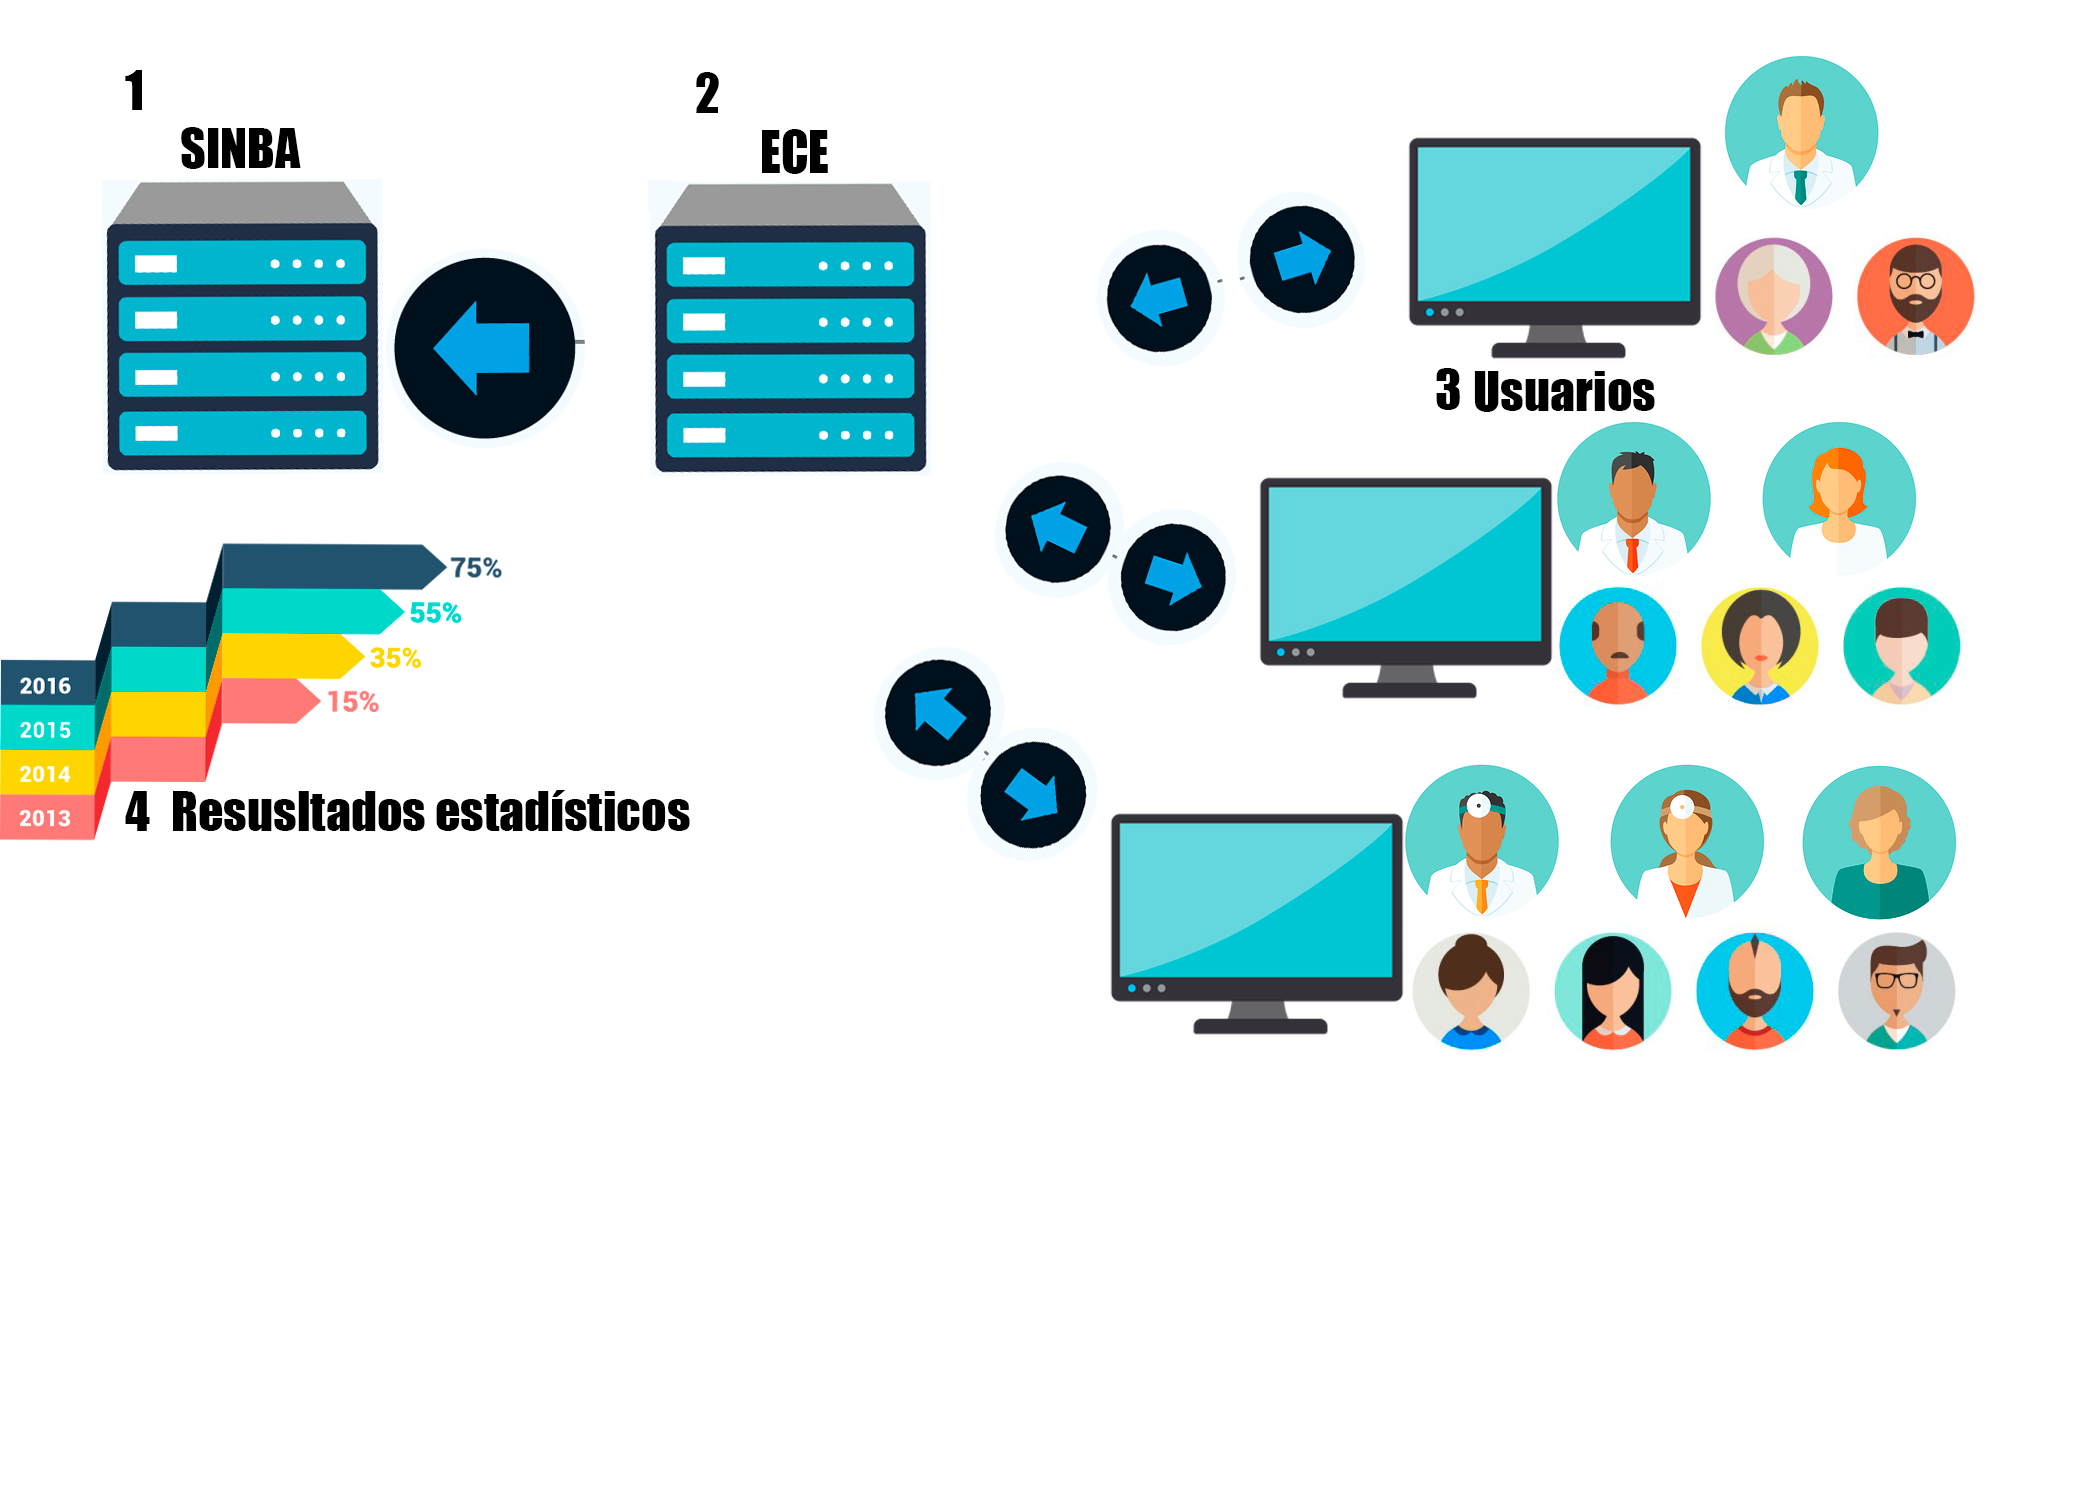
\includegraphics[scale=.1]{lib/assets/propuesta}
  \caption{Propuesta Técnica}
\end{figure}
\subsection{Descripción de la propuesta técnica}
1.Sistema Nacional de Información Básica en Materia de Salud (SINBA). Es creada por el gobierno federal para poder concentrar la información de los treinta y dos estados federativos sobre materia de salud.

2. Expediente Clínico Electrónico (ECE). Se crea a partir de la necesidad de poder agilizar el proceso de atención de las personas, además de poder concentrar toda la información del estado de Chiapas en materia de salud para así poder ser exportarlos a SIMBA.

3. Usuarios. Los usuarios favorecidos con la creación de dicho sistema serán principalmente los médicos, personal de salud en general y por consecuente los pacientes. reduciendo el tiempo del proceso de atención.


\section{Impácto}

\subsection{Impácto Social}

Según estimaciones oficiales, la aplicación del ECE podría representar el ahorro de 38 mil millones de pesos para el sistema de salud, debido a que se contrarrestarían posibles negligencias médicas, retrasos en la atención, cirugías, robo y desperdicio de medicamento, entre otros. Esto debido a que la falta de información clínica retrasa la atención y puede ser la causa de errores médicos. Esta evolución tecnológica permitirá aumentar la productividad en 20 por ciento; reducir los tiempos y días de espera para consultar en 60 por ciento y ahorros de hasta el 80 por ciento en papelería; reducir los tiempos para cirugía que llegan a ser de hasta 62 días, así como disminuir el desperdicio de medicamento. Además de colocar a México a la altura de otros países que ya implementan este mecanismo. Manual del Expediente Clínico Electrónico. Dirección General de Información en Salud. Secretaría de Salud. México, 2011.
Pacientes con estabilidad respiratoria, hemodinámica y neurológica, el tiempo de espera máximo debe ser de 60 minutos; y verde, pacientes con estabilidad respiratoria, hemodinámica y neurológica, con aspecto saludable y sin riesgo evidente de complicaciones, el tiempo de espera es de hasta cuatro horas. (Chiapas, 2017)
La implementación de un expediente clínico en el estado de Chiapas representaría un gran ahorro económico, tiempo y así como agilizar la atención de cada uno de los pacientes. Actualmente el tiempo de espera para los pacientes en los hospitales llega a ser de cuatro horas, siendo este demasiado tiempo, el cual las personas pudiesen ocupar para realizar sus actividades económicas ya que en el estado un gran porcentaje de la población vive al día con lo poco que gana durante una jornada laborar, siendo esta de una ganancia no estable. Se espera reducir el tiempo de espera en un 80\% con el expediente clínico electrónico.

\subsection{Impácto Tecnológico}
El impácto Tecnológico principal del proyecto será que se desarrolle a las necesidades de la secretaria de salud del estado de Chiapas, siendo una de estas que funcione de manera online y offline, además que pueda contar con una gran escalabilidad ya que es pensado para manejar grandes cantidades de información, datos estadísticos y por supuesto con la mayor seguridad posible.  Con ello se pretende eliminar en su mayoría la duplicidad de los datos o la perdida da de los mismos. Además, se ayudará a aplicar acciones preventivas en la población. Se tendrá un acceso más rápido a la información para la ayuda de investigaciones y desarrollo de la salud en el estado.

\section{Metodología en cascada}
    \subsection{Descripción de la metodología}
      Es el enfoque metodológico que ordena rigurosamente las etapas del ciclo de vida
      del software, de tal forma que el inicio de cada etapa debe esperar a la finalización
      de la inmediatamente anterior (Figura \ref{metodologia})

      \begin{figure}[h]
        \centering
        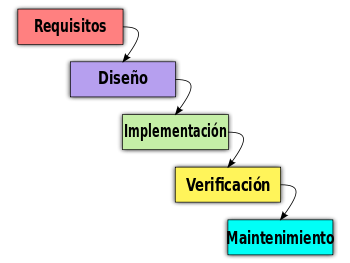
\includegraphics[scale=.7]{lib/assets/cascada}
        \caption{Diagrama de la metodología.}
        \label{metodologia}
      \end{figure}


De esta forma, cualquier error de diseño detectado en la etapa de prueba conduce
necesariamente al rediseño y nueva programación del código afectado, aumentando
los costos del desarrollo.


  \subsection{Justificación de metodología}

  La decisión por el cual se eligió esta metodología fue por la menera en la que se está trabajando con los contribuyentes exteriores, de parte de Secretaria de Salud recibimos la parte de analizis y requerimientos del sistema, por nuestra parte trabajaremos lo que es la interoperabilidad de los Sistemas de expediente Clínico.
        \subsection{Pasos de la metodología}
            \subsubsection{ Requisitos del software}
      \begin{center}
        \begin{minipage}{0.9\linewidth}
          \vspace{5pt}%margen superior
          {\small
                En esta fase se hace un análisis de las necesidades del cliente para determinar las características del software a desarrollar, y se especifica todo lo que debe hacer el sistema sin entrar en detalles técnicos. Hay que ser especialmente cuidadoso en esta primera fase, ya que en este modelo no se pueden añadir nuevos requisitos en mitad del proceso de desarrollo.
          }
          \begin{flushright}
            (\author{En qué consiste el modelo en cascada.},
            \citeyearNP{https://openclassrooms.com/courses/gestiona-tu-proyecto-de-desarrollo/en-que-consiste-el-modelo-en-cascada}: 2017)
          \end{flushright}
            \vspace{5pt}%margen inferior de la minipage
        \end{minipage}
      \end{center}
            \subsubsection{Diseño}
            \begin{center}
              \begin{minipage}{0.9\linewidth}
                \vspace{5pt}%margen superior
                {\small
                En esta etapa se describe la estructura interna del software, y las relaciones entre las entidades que lo componen.

                Descompone y organiza el sistema en elementos que puedan elaborarse por separado, aprovechando las ventajas del desarrollo en equipo. Como resultado surge el SDD (Documento de Diseño del Software), que contiene la descripción de la estructura relacional global del sistema y la especificación de lo que debe hacer cada una de sus partes, así como la manera en que se combinan unas con otras.
                }
                \begin{flushright}
                  (\author{En qué consiste el modelo en cascada.},
                  \citeyearNP{https://openclassrooms.com/courses/gestiona-tu-proyecto-de-desarrollo/en-que-consiste-el-modelo-en-cascada}: 2017)
                \end{flushright}
                  \vspace{5pt}%margen inferior de la minipage
              \end{minipage}
            \end{center}
            \subsubsection{Implementación}
            \begin{center}
              \begin{minipage}{0.9\linewidth}
                \vspace{5pt}%margen superior
                {\small

                En esta fase se programan los requisitos especificados haciendo uso de las estructuras de datos diseñadas en la fase anterior.La programación es el proceso que lleva de la formulación de un problema de computación, a un programa que se ejecute produciendo los pasos necesarios para resolver dicho problema.

                Al programar, tenemos que realizar actividades como el análisis de las condiciones, la creación de algoritmos,  y la implementación de éstos en un lenguaje de programación específico.
                }
                \begin{flushright}
                  (\author{En qué consiste el modelo en cascada.},
                  \citeyearNP{https://openclassrooms.com/courses/gestiona-tu-proyecto-de-desarrollo/en-que-consiste-el-modelo-en-cascada}: 2017)
                \end{flushright}
                  \vspace{5pt}%margen inferior de la minipage
              \end{minipage}
            \end{center}
            \subsubsection{Verificación}
            \begin{center}
              \begin{minipage}{0.9\linewidth}
                \vspace{5pt}%margen superior
                {\small
                Como su propio nombre indica, una vez se termina la fase de implementación se verifica que todos los componentes del sistema funcionen correctamente y cumplen con los requisitos.

                El objetivo de las pruebas es el de obtener información de la calidad del software, y sirven para: encontrar defectos o bugs, aumentar la calidad del software, refinar el código previamente escrito sin miedo a romperlo o introducir nuevos bugs, etc.
                }
                \begin{flushright}
                  (\author{En qué consiste el modelo en cascada.},
                  \citeyearNP{https://openclassrooms.com/courses/gestiona-tu-proyecto-de-desarrollo/en-que-consiste-el-modelo-en-cascada}: 2017)
                \end{flushright}
                  \vspace{5pt}%margen inferior de la minipage
              \end{minipage}
            \end{center}

            \subsubsection{Instalación y mantenimiento
}
            \begin{center}
              \begin{minipage}{0.9\linewidth}
                \vspace{5pt}%margen superior
                {\small

                Una vez se han desarrollado todas las funcionalidades del software y se ha comprobado que funcionan correctamente, se inicia la fase de instalación y mantenimiento. Se instala la aplicación en el sistema y se comprueba que funcione correctamente en el entorno en que se va a utilizar.

                A partir de ahora hay que asegurarse de que el software funcione y hay que destinar recursos a mantenerlo. El mantenimiento del software consiste en la modificación del producto después de haber sido entregado al cliente, ya sea para corregir errores o para mejorar el rendimiento o las características.


                }
                \begin{flushright}
                  (\author{En qué consiste el modelo en cascada.},
                  \citeyearNP{https://openclassrooms.com/courses/gestiona-tu-proyecto-de-desarrollo/en-que-consiste-el-modelo-en-cascada}: 2017)
                \end{flushright}
                  \vspace{5pt}%margen inferior de la minipage
              \end{minipage}
            \end{center}

    \subsection{Pasos de la metodología aplicada en el proyecto}
          \subsubsection{Requisitos del software}
          \begin{itemize}
            \item Debe recibir, registrar y administrar documentación clínica externa a través de mecanismos de interoperabilidad.
            \item Debe recibir, almacenar y mostrar resultados clínicos de estudios de gabinete de fuentes externas como pueden ser las imágenes radiológicas, los archivos de onda de trazados, electrocardiográma, sistemas de farmacia, por medio de mecanismos de interoperabilidad.
            \item Debe enviar y recibir información, metadatos, imágenes, resultados de laboratorio y documentos por medio de interoperabilidad.
            \item Debe soportar interoperabilidad semántica mediante el uso de terminologías y modelos estándar para habilitar la interoperabilidad y promover la consistencia de la información compartida.
            \item Debe apegarse a los protocolos definidos para interactuar con Sistemas Estatales, Institucionales o Nacionales de interoperabilidad de acuerdo a los lineamientos que para este fin sean publicados por la Secretaría de Salud.

          \end{itemize}

          \subsubsection{Diseño}

          \begin{figure}[h]
            \centering
            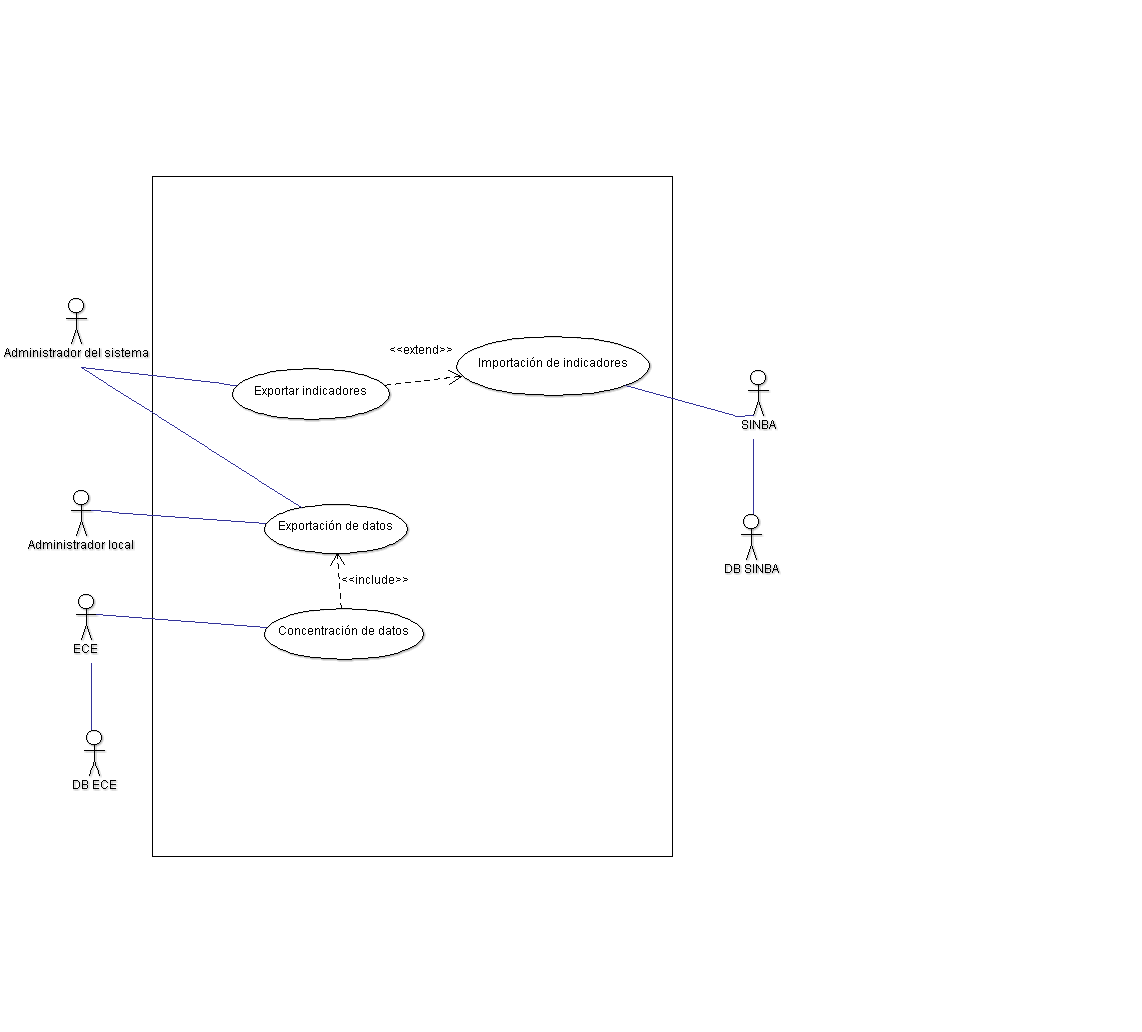
\includegraphics[scale=.3]{lib/assets/casodeuso}
            \caption{Diagrama de caso de uso.}
            \label{metodologia}
          \end{figure}

            \begin{figure}[h]
             \centering
              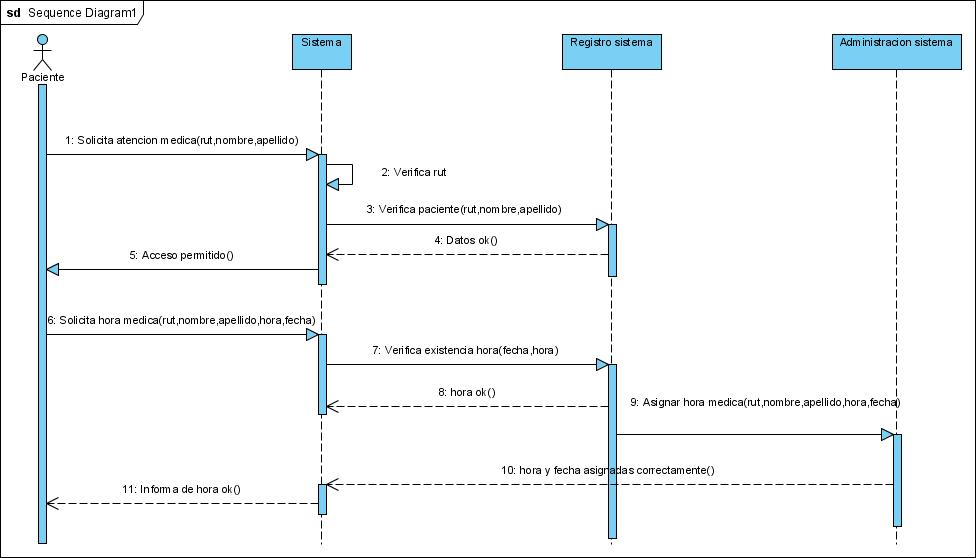
\includegraphics[scale=.5]{lib/assets/secuencia}
              \caption{Diagrama de caso de uso.}
              \label{metodologia}
            \end{figure}
          \subsubsection{Implementación}
          \subsubsection{Verificación}
          \subsubsection{Instalación y mantenimiento}
